\subsection{Entraînement}

L'entraînement du modèle est un problème d'optimisation.
Étant donné une fonction qui mesure la dissimilarité entre la sortie du modèle et la cible,
le but est de trouver les valeurs des paramètres qui minimisent cette fonction.

\subsubsection{Algorithmes d'optimisation}

Plusieurs algorithmes d'optimisation sont utilisés pour entraîner les modèles de \gls{dl}.
La majorité d'entre eux sont basés sur l'algorithme du gradient.
C'est le cas de l'algorithme d'optimisation Adam \cite{Kingma_Ba_2017} que nous avons utilisé.
Il s'agit d'un algorithme itératif qui met à jour les paramètres du modèle à chaque itération.
% \begin{eqnarray}
%     \label{eq.adam}
%     m_w^{(t+1)} &=& m_w^{(t)}+\left(1-\beta_1\right) \nabla_w L^{(t)} \\
%     v_w^{(t+1)} &=& v_w^{(t)}+\left(1-\beta_2\right)\left(\nabla_w L^{(t)}\right)^2 \\
%     \hat{m}_w&=&\frac{m_w^{(t+1)}}{1-\beta_1^t} \\
%     \hat{v}_w&=&\frac{v_w^{(t+1)}}{1-\beta_2^t} \\
%     w^{(t+1)} &=& w^{(t)}-\eta \frac{\hat{m}_w}{\sqrt{\hat{v}_w}+\epsilon}
% \end{eqnarray}
Son comportement est contrôlé par plusieurs hyperparamètres,
mais le seul que nous avons modifié est le taux d'apprentissage \(\eta\) que nous avons initialisé à
\(3\cdot 10^{-4}\), une valeur récurrente dans la littérature~\cite{islam2022face,lu2023deformable}.

Pour accélérer l'entraînement, il est fait d'une manière \emph{stochastique}.
Cela signifie que la fonction de perte est estimée 
sur un sous-ensemble des données d'entraînement qu'on appelle un \emph{lot}.
La taille du lot peut avoir un grand impact sur la performance du modèle.
Dans notre cas, nous avons utilisé des lots de 256 paires de phrases%
\footnote{%
  La plus grande taille de lot compatible avec la mémoire de la carte graphique utilisée.
}.


\subsubsection{Contre-mesures au sur-apprentissage}

Le sur-apprentissage est un problème courant dans l'entraînement des modèles de \gls{dl}.
Pour mitiger ce risque, nous avons utilisé plusieurs techniques.
L'une d'entre elles est le \emph{\foreignlanguage{english}{dropout}}.
Il s'agit d'une technique de régularisation 
qui consiste à ignorer aléatoirement une fraction \(p_{\mathrm{drop}}\) des valeurs d'une couche.

Une autre méthode de régularisation est la majoration de la norme des vecteurs de plongement.
Cela permet de contraindre les paramètres des couches de plongement lexical
et, par conséquent, de réduire sa puissance de représentation.



\subsubsection{Réglage des hyperparamètres}

Les hyperparamètres sont les paramètres du modèle qui ne sont pas appris durant l'entraînement.
Dans notre cas, ces paramètres incluent les dimensions de plongement, 
la taille du vocabulaire, le nombre de couches du transformeur, 
le nombre de têtes d'attention, 
le \emph{\foreignlanguage{english}{dropout}} et la taille des lots d'entraînement.
Leurs valeurs sont souvent fixées par l'utilisateur.
Cependant, elles peuvent avoir un impact significatif sur les performances du modèle.
Elles sont donc souvent choisies en explorant systématiquement l'espace des possibilités.
Cette exploration peut se faire d'une manière exhaustive ou aléatoire.

\begin{figure}[htb]
    \begin{center}
        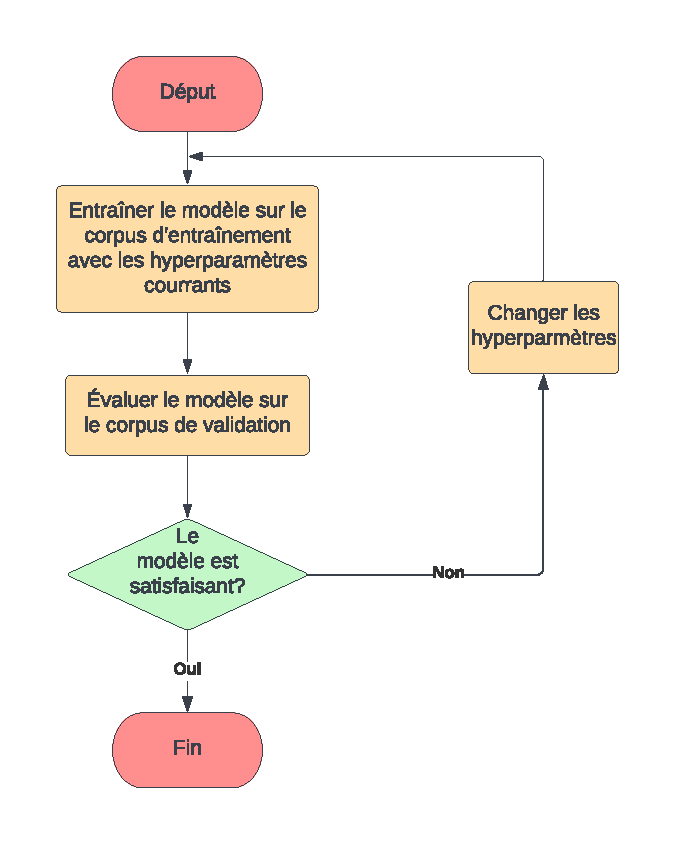
\includegraphics[width=7cm]{assets/pdf/Training.pdf}
    \end{center}
    \caption{Organigramme de la phase d'entraînement.}
    \label{fig.training}
\end{figure}

Le problème de réglage des hyperparamètres est aussi un problème d'optimisation.
Or, il est souvent de nature discrète ou mixte, car les hyperparamètres ne sont pas nécessairement continus.
Cela rend l'optimisation beaucoup plus difficile.
La fonction objectif est généralement calculée à partir du jeu de données de validation.

Le processus d'entraînement dans sa totalité est illustré par la Figure~\ref{fig.training}.
On note sur la figure que le réglage des hyperparamètres n'est effectué 
que si le modèle entraîné avec la combinaison initiale d'hyperparamètres n'est pas satisfaisant.
Sinon, la condition d'arrêt est atteinte et le modèle est utilisé pour la phase d'évaluation.

Il est important de noter que le corpus de test est particulièrement important 
dans le cas où le réglage des hyperparamètres est effectué.
Dans ce cas, il est possible que le sur-apprentissage se produise simultanément 
sur le corpus d'entraînement et celui de validation.
Le corpus de test est donc la seule manière d'obtenir une estimation non biaisée de la performance du modèle.